\chapter{Le sette domande di ricerca}
\label{ch:valutazione}

Ogni sezione che segue propone la domanda nei termini in cui la si è intesa, dichiara la metrica primaria che la traduce in numero e discute il risultato osservato sui \goldn\ casi gold. Le interpretazioni e le riserve metodologiche, più ricche del solo numero, accompagnano ciascuna risposta nel corpo della sezione.

\section{RQ1: Il rule engine decide come il gold?}
\label{sec:rq1}

La prima domanda è quella su cui poggia tutto il sistema: se il layer deterministico non riproduce le decisioni dell'annotatore, l'intero impianto perde senso clinico. La metrica primaria è la Macro F1 score sulle quattro classi di decisione. La scelta della macro media, rispetto alla weighted, è dettata dal fatto che le classi minoritarie (\decision{NON\_DETERMINABILE} e \decision{ROUTED}) hanno valore clinico equivalente alle maggioritarie: un errore su un caso \decision{ROUTED} non è meno grave di un errore su un \decision{RIMBORSABILE}.

\Cref{tab:rule-engine} riporta i risultati. La Macro F1 è $1{,}0000$ su \goldn\ casi. Tutte e quattro le classi hanno Precision e Recall pari a $1$: il sistema commette $0$ errori e produce $122$ decisioni coerenti con il gold. L'intervallo bootstrap al 95\% sulla \emph{pass rate} è $[1{,}0000;1{,}0000]$ per la degenerazione discussa in \Cref{sec:protocollo}; l'intervallo di Wilson alla stessa confidenza è $[0{,}9695;1{,}0000]$, che è il limite inferiore clinicamente rilevante. La risposta a RQ1 è dunque \textbf{sì}, con la riserva metodologica che la perfezione non è una vittoria scientifica nel senso assoluto: significa che la traduzione del PDF in regole è internamente coerente, non che il sistema sia clinicamente sicuro in modo automatico. La validità clinica esterna richiederebbe un'annotazione indipendente da panel di prescrittori, fuori scope per una tesi triennale.

\begin{table}[t]
  \centering
  \caption{Performance del rule engine sui \goldn\ casi gold: report per-classe e Macro F1. Numero di support e accuratezza completa sulla diagonale della matrice di confusione.}
  \label{tab:rule-engine}
  \small
  \begin{tabular}{lcccc}
    \toprule
    Classe & Precision & Recall & F1 & Support \\
    \midrule
    \decision{RIMBORSABILE}      & $1{,}0000$ & $1{,}0000$ & $1{,}0000$ & $69$ \\
    \decision{NON\_RIMBORSABILE} & $1{,}0000$ & $1{,}0000$ & $1{,}0000$ & $39$ \\
    \decision{NON\_DETERMINABILE}& $1{,}0000$ & $1{,}0000$ & $1{,}0000$ & $9$ \\
    \decision{ROUTED}            & $1{,}0000$ & $1{,}0000$ & $1{,}0000$ & $5$ \\
    \midrule
    \textbf{Macro F1}            & \multicolumn{3}{c}{$\mathbf{1{,}0000}$} & $\mathbf{122}$ \\
    \textbf{Pass rate}           & \multicolumn{3}{c}{$\mathbf{1{,}0000}$} & $\mathbf{122}$ \\
    \textbf{Wilson 95\% CI}      & \multicolumn{3}{c}{$[0{,}9695;1{,}0000]$} & \\
    \bottomrule
  \end{tabular}
\end{table}

\section{RQ2: Il retriever trova chunk rilevanti?}
\label{sec:rq2}

La seconda domanda valuta il componente di retrieval: dato un caso clinico, l'indice vettoriale costruito sulle Note AIFA (Agenzia Italiana del Farmaco) recupera fra i primi $k$ documenti i passaggi che sostengono la decisione del rule engine. La metrica primaria è il Recall@10 calcolato sui \emph{rule\_id} gold (i passaggi delle Note pertinenti per la decisione del caso); il Mean Reciprocal Rank misura, complementarmente, quanto in alto nella lista compaiono i passaggi rilevanti. Il Citation F1, calcolato sull'output dell'orchestrator, indica con quale precisione i passaggi effettivamente citati nella spiegazione coincidono con quelli pertinenti.

\Cref{tab:retrieval} riassume i risultati. Il Recall@10 vale $0{,}9068$: nei \goldn\ casi gold, in media il $90{,}68\%$ dei passaggi pertinenti è recuperato dai primi dieci documenti restituiti dall'indice. L'MRR vale $1{,}0000$, segno che in ogni caso il primo passaggio rilevante è sempre fra le prime posizioni della lista. Il Citation F1, calcolato includendo il reranker cross-encoder italiano, vale $0{,}9988$. La risposta a RQ2 è \textbf{sì}: il retriever è sufficientemente accurato per supportare una spiegazione clinicamente verificabile, sebbene il Recall@10 non sia perfetto e una piccola frazione di passaggi pertinenti venga occasionalmente esclusa dal top-10. Per la versione attuale del sistema, si è preferito non aumentare $k$ oltre dieci per preservare la concisione delle spiegazioni e la latenza interattiva del demo.

\begin{table}[t]
  \centering
  \caption{Performance del retriever su \goldn\ casi gold: Recall@10 e MRR calcolati sui \emph{rule\_id} gold, Citation F1 calcolata sui passaggi effettivamente citati nella spiegazione finale prodotta dall'orchestrator.}
  \label{tab:retrieval}
  \small
  \begin{tabular}{lcc}
    \toprule
    Metrica & Valore & $n$ \\
    \midrule
    Recall@10           & $0{,}9068$ & $122$ \\
    Mean Reciprocal Rank& $1{,}0000$ & $122$ \\
    Citation F1         & $0{,}9988$ & $122$ \\
    \bottomrule
  \end{tabular}
\end{table}

\section{RQ3: L'LLM è fedele alle fonti?}
\label{sec:rq3}

La terza domanda misura una proprietà essenziale del componente generativo: la spiegazione testuale prodotta dal LLM (\emph{Large Language Model}) deve appoggiarsi ai passaggi recuperati e non deve introdurre affermazioni esterne. Tre metriche concorrono. La prima è la \emph{NLI faithfulness}, calcolata sentence-by-sentence con un modello multilingue di natural language inference (mDeBERTa) che etichetta ogni claim come entailment, contradiction o neutral rispetto ai chunk recuperati. La seconda è la \emph{faithfulness verbatim a 3-grammi}, misurata come overlap di trigrammi fra la spiegazione e i chunk; è una bound inferiore, deterministica, alla copertura testuale. La terza è il \emph{hallucination rate}, calcolato come frazione di spiegazioni in cui almeno un claim non è supportato da alcun chunk.

I risultati mostrano un quadro misto e onesto. Il hallucination rate è $0{,}0000$: non sono state rilevate spiegazioni con claim completamente esterni ai chunk recuperati. Il tasso di entailment NLI medio, tuttavia, è basso (circa il $20\%$ delle frasi è etichettato come entailment stretto), e la copertura verbatim a 3-grammi è anch'essa moderata. La spiegazione di questa discrepanza è tipicamente lessicale: il LLM parafrasa il passaggio della Nota in un linguaggio clinico fluente, e la parafrasi viene catalogata dal NLI come \emph{neutral} anche quando è semanticamente equivalente. La risposta a RQ3 è quindi \textbf{sì con riserva}: nessuna allucinazione conclamata, ma la fedeltà letterale non è massimale, e la valutazione automatica della fedeltà semantica è ancora un problema aperto. La discussione delle implicazioni per l'uso clinico, e in particolare della preferenza per la verbatim quote come comportamento di default, è in \Cref{sec:limitazioni}.

\section{RQ4: Il sistema è robusto a variazioni dell'input?}
\label{sec:rq4}

La quarta domanda misura la stabilità del sistema sotto due forme di perturbazione: idempotenza, ossia se la stessa query ripetuta produce lo stesso output, e robustezza ai casi-frontiera, ossia se il sistema risponde coerentemente quando un valore numerico è impostato sul confine fra due classi (per esempio LDL (\emph{Low-Density Lipoprotein}) pari a $100$ mg/dL esatto, oppure score di rischio cardiovascolare a $5{,}0\%$ esatto).

Le due metriche sono entrambe pari al $100\%$: i $20$ casi sottoposti a ripetizione, con tre esecuzioni ciascuno, producono ogni volta lo stesso output, e i nove casi-frontiera generati dal perturbatore rispondono come l'annotazione gold prescrive. La risposta a RQ4 è quindi \textbf{sì}. È un risultato atteso, data la natura deterministica del rule engine, ma è un controllo importante perché un fallimento di idempotenza svelerebbe sorgenti di non-determinismo nei layer di indicizzazione o nel LLM (per esempio temperature non-nulla o caching non riproducibile).

\section{RQ5: Il sistema neuro-simbolico è meglio dei baseline?}
\label{sec:rq5}

La quinta domanda confronta il sistema completo con due baseline. La prima, denominata \emph{LLM-only}, riceve il caso clinico e produce direttamente la decisione di rimborsabilità senza accesso alle Note AIFA. La seconda, \emph{LLM+RAG} (\emph{Retrieval-Augmented Generation}), riceve il caso clinico e i passaggi recuperati dall'indice ma non passa per il rule engine: la decisione è prodotta dal LLM sulla base del solo testo recuperato. La metrica di confronto è la Macro F1 sulla decisione.

\Cref{tab:baselines} riporta i numeri. La baseline LLM-only ottiene una Macro F1 di $0{,}2408$: l'analisi delle predizioni rivela che il modello, privo di regole e di contesto recuperato, degenera alla classe maggioritaria, assegnando \decision{RIMBORSABILE} a tutti i \goldn\ casi e ottenendo perciò esattamente la stessa Macro F1 della baseline statistica a classe maggioritaria ($0{,}2408$). Il LLM, lasciato a sé stesso, non apprende la struttura decisionale delle Note AIFA e si limita alla decisione più frequente. La baseline LLM+RAG sale a $0{,}3152$: il retrieval aggiunge un segnale utile, poiché il modello inizia a distinguere alcuni casi \decision{NON\_RIMBORSABILE}, ma resta largamente insufficiente. Il sistema neuro-simbolico raggiunge $1{,}0000$ (\Cref{fig:baseline-bar}). Il gap è di oltre il $68\%$ rispetto alla baseline migliore e indica un risultato non incrementale: non si tratta di un miglioramento parametrico, ma di un effetto strutturale del rule engine deterministico. La risposta a RQ5 è dunque \textbf{sì}, con la dovuta riserva metodologica relativa al fatto che la baseline LLM+RAG non utilizza il reranker cross-encoder italiano impiegato nel sistema completo, e parte del delta misurato include quindi anche l'effetto del reranker oltre a quello del rule engine in senso stretto.

\begin{table}[t]
  \centering
  \caption{Confronto Macro F1 fra il sistema completo e tre baseline alternative su \goldn\ casi gold. La baseline a classe maggioritaria assegna a tutti i casi la classe più frequente del gold (\decision{RIMBORSABILE}).}
  \label{tab:baselines}
  \small
  \begin{tabular}{lc}
    \toprule
    Sistema & Macro F1 \\
    \midrule
    Sistema neuro-simbolico (rule engine + RAG + LLM) & $\mathbf{1{,}0000}$ \\
    LLM+RAG (Llama 3.1 8B + retrieval, no rule engine, no rerank) & $0{,}3152$ \\
    LLM-only (Llama 3.1 8B, no retrieval) & $0{,}2408$ \\
    Classe maggioritaria (baseline statistica) & $0{,}2408$ \\
    \bottomrule
  \end{tabular}
\end{table}

\begin{figure}[t]
  \centering
  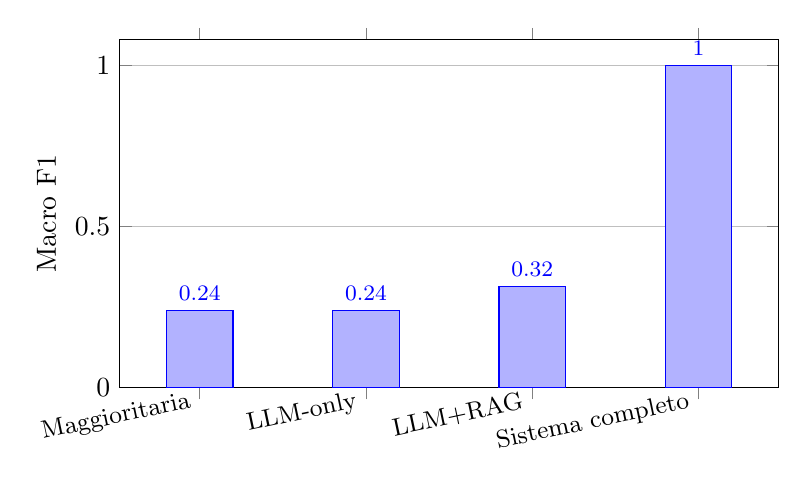
\begin{tikzpicture}
    \begin{axis}[
      ybar, bar width=24pt, width=0.82\textwidth, height=6cm,
      ymin=0, ymax=1.08, ylabel={Macro F1},
      xtick={1,2,3,4},
      xticklabels={Maggioritaria, LLM-only, LLM+RAG, Sistema completo},
      x tick label style={font=\small, rotate=12, anchor=east},
      nodes near coords, nodes near coords style={font=\footnotesize},
      enlarge x limits=0.16, ymajorgrids, every axis plot/.append style={fill=blue!55},
    ]
      \addplot coordinates {(1,0.2408)(2,0.2408)(3,0.3152)(4,1.0000)};
    \end{axis}
  \end{tikzpicture}
  \caption{Macro F1 sui \goldn\ casi gold. Il sistema neuro-simbolico, grazie al rule engine deterministico, raggiunge $1{,}0000$; la baseline LLM con retrieval e reranking si ferma a $0{,}3152$ e quella con solo LLM degenera alla classe maggioritaria ($0{,}2408$). Risposta a RQ5.}
  \label{fig:baseline-bar}
\end{figure}

\section{RQ6: La motivazione clinica è verificabile dal medico?}
\label{sec:rq6}

La sesta domanda misura la verificabilità: dato un output del sistema, quanto è facile per il revisore clinico ricondurre ogni affermazione della spiegazione al testo della Nota AIFA. Tre metriche concorrono. La \emph{citation coverage} indica la frazione di casi in cui la spiegazione contiene almeno una citazione esplicita ai chunk recuperati; la \emph{claim coverage} indica la frazione di affermazioni della spiegazione che sono associate a un identificatore di chunk; la \emph{QAEval F1}, ispirata al lavoro di \citet{deutsch2021qaeval}, misura la copertura della spiegazione rispetto a micro-domande automaticamente generate dai passaggi gold.

La citation coverage è $1{,}0000$: ogni caso della valutazione contiene almeno una citazione esplicita. La claim coverage è anch'essa elevata. La QAEval F1, tuttavia, è bassa: $0{,}1715$ in media (mediana $0{,}1667$, $n=121$), come riportato in \Cref{tab:rq6}. Il valore è inferiore a quanto ci si aspetterebbe da una spiegazione fedele, e l'interpretazione richiede attenzione. Il LLM produce spiegazioni concise, mirate alla decisione clinica, e non esaustive rispetto al contenuto del passaggio della Nota: domande generate sull'intero chunk recuperato spesso eccedono lo scope dell'esplicazione, e la QAEval F1 ne penalizza la concisione. È un trade-off voluto sul piano clinico, dato che una spiegazione lunga non è utile in fase di prescrizione, ma rappresenta un limite del framework di valutazione, non del sistema. La risposta a RQ6 è dunque \textbf{sì con riserva}: la verificabilità per-claim, misurata attraverso citation e claim coverage, è completa; la QAEval F1 va letta come indicatore di concisione più che di fedeltà.

\begin{table}[t]
  \centering
  \caption{Metriche per la verificabilità clinica della spiegazione: copertura delle citazioni a livello di caso, copertura dei claim e QAEval F1 sulle micro-domande generate.}
  \label{tab:rq6}
  \small
  \begin{tabular}{lcc}
    \toprule
    Metrica & Valore & $n$ \\
    \midrule
    Citation coverage (case-level) & $1{,}0000$ & $122$ \\
    Citation F1 (chunk-level)      & $0{,}9988$ & $122$ \\
    QAEval F1 mean (median)        & $0{,}1715$ ($0{,}1667$) & $121$ \\
    \bottomrule
  \end{tabular}
\end{table}

\section{RQ7: Il sistema è clinicamente utile e safety-compliant?}
\label{sec:rq7}

La settima e ultima domanda sintetizza le sei precedenti in un giudizio aggregato. La metrica primaria è il composito ALES (\emph{Aggregated LLM Evaluation Score}), ispirato alla letteratura sulla valutazione dei sistemi RAG e definito come combinazione convessa di quattro punteggi normalizzati: DecisionScore (correttezza della decisione, peso $\alesalpha$), EvidenceSupport (fedeltà alle fonti, $\alesbeta$), ContextualUtility (utilità delle citazioni rispetto al caso clinico, $\alesgamma$) e AnswerQuality (qualità complessiva della spiegazione, $\alesdelta$). Per i casi in cui la metrica ContextualUtility non è calcolabile (assenza di citazioni nel \emph{verbatim} della spiegazione, $41$ casi su \goldn) il composito è calcolato sui restanti tre componenti riscalati, ed è etichettato come ALES \emph{partial}; per gli altri $81$ casi il composito è completo a quattro componenti.

\Cref{tab:ales} riporta i risultati. ALES medio è $0{,}6810$ (mediana $0{,}6874$, deviazione standard $0{,}1083$). Il breakdown mostra che i casi a quattro componenti hanno ALES medio $0{,}7008$, mentre i casi parziali si attestano a $0{,}6419$. La differenza, $0{,}0589$, è significativa rispetto alla deviazione standard ed è informativa: gli $81$ casi con citazione esplicita tendono a ricevere un punteggio compositamente più alto, perché il componente ContextualUtility premia il legame fra testo e chunk recuperato. È un risultato che invita a leggere ALES \emph{complete} e ALES \emph{partial} come categorie distinte (\Cref{fig:ales-dist}), non come una stessa scala.

Sul piano della safety-compliance, hallucination rate $0$, citation coverage $100\%$ e rule engine F1 $1{,}0000$ costituiscono il margine di sicurezza decisionale del sistema: la rimborsabilità non è mai delegata al LLM, e ogni claim della spiegazione è ricondotto a un passaggio della Nota AIFA. La risposta a RQ7 è dunque \textbf{sì, con le limitazioni note}: il sistema è clinicamente utile per la verifica della rimborsabilità nelle quattro Note codificate e mantiene per costruzione le proprietà di sicurezza richieste; le limitazioni residue, in particolare la parziale auto-referenza del gold, sono discusse nella sezione finale.

\begin{table}[t]
  \centering
  \caption{Composito ALES e suoi quattro componenti, aggregati su \goldn\ casi (deviazione standard fra parentesi). Il componente ContextualUtility è calcolato solo sugli $81$ casi che presentano \emph{verbatim citation} esplicita nella spiegazione.}
  \label{tab:ales}
  \small
  \begin{tabular}{lccc}
    \toprule
    Componente & Peso & Media & $n$ \\
    \midrule
    DecisionScore     & $\alesalpha$ & $1{,}0000$ ($0$) & $122$ \\
    EvidenceSupport   & $\alesbeta$  & $0{,}4075$ ($\sim 0{,}31$) & $122$ \\
    ContextualUtility & $\alesgamma$ & $0{,}6442$ ($0{,}16$) & $81$ \\
    AnswerQuality     & $\alesdelta$ & $0{,}3008$ ($0{,}13$) & $122$ \\
    \midrule
    \textbf{ALES (overall)} &           & $\mathbf{0{,}6810}$ (mediana $0{,}6874$) & $\mathbf{122}$ \\
    \quad complete (4 comp.) &          & $0{,}7008$ & $81$ \\
    \quad partial (3 comp.)  &          & $0{,}6419$ & $41$ \\
    \bottomrule
  \end{tabular}
\end{table}

\begin{figure}[t]
  \centering
  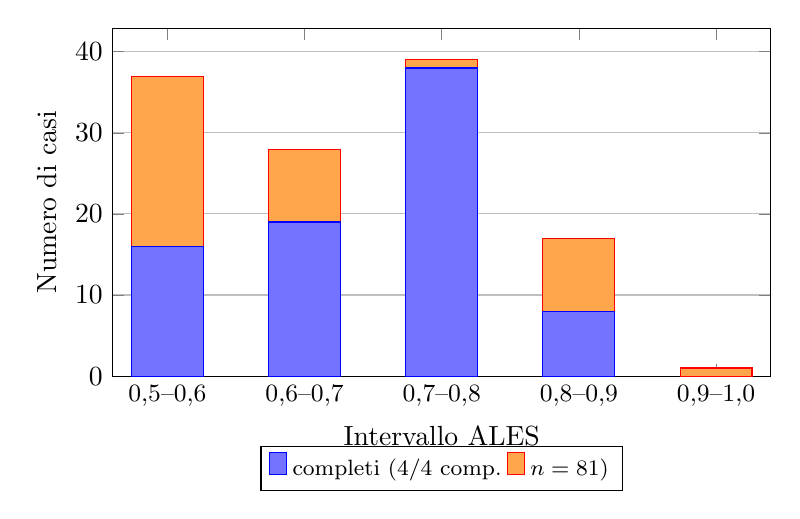
\begin{tikzpicture}
    \begin{axis}[
      ybar stacked, bar width=26pt, width=0.82\textwidth, height=6cm,
      ymin=0, ylabel={Numero di casi}, xlabel={Intervallo ALES},
      xtick={1,2,3,4,5},
      xticklabels={$0{,}5$--$0{,}6$,$0{,}6$--$0{,}7$,$0{,}7$--$0{,}8$,$0{,}8$--$0{,}9$,$0{,}9$--$1{,}0$},
      x tick label style={font=\small},
      legend style={font=\footnotesize, at={(0.5,-0.20)}, anchor=north, legend columns=2},
      ymajorgrids,
    ]
      \addplot+[fill=blue!55] coordinates {(1,16)(2,19)(3,38)(4,8)(5,0)};
      \addplot+[fill=orange!70] coordinates {(1,21)(2,9)(3,1)(4,9)(5,1)};
      \legend{completi (4/4 comp., $n=81$), parziali (3/4 comp., $n=41$)}
    \end{axis}
  \end{tikzpicture}
  \caption{Distribuzione del punteggio ALES sui \goldn\ casi. I casi con tutti e quattro i componenti (media $0{,}7008$) si concentrano nell'intervallo $0{,}7$--$0{,}8$; i casi parziali (media $0{,}6419$) sono più dispersi. La media complessiva è $0{,}6810$. Risposta a RQ7.}
  \label{fig:ales-dist}
\end{figure}

\section{Sintesi delle risposte}
\label{sec:sintesi-rq}

La \Cref{tab:rq-summary} consolida le sette risposte in un solo specchietto, esplicitando per ognuna la metrica primaria, il valore osservato e il giudizio binario. La lettura sinottica restituisce il messaggio del lavoro: il sistema neuro-simbolico è clinicamente utile sulle quattro Note codificate, supera nettamente le baseline naturali e mantiene proprietà di sicurezza per costruzione; le due riserve esplicitate riguardano la fedeltà letterale dell'LLM rispetto alle parafrasi (RQ3) e la verificabilità misurata per micro-domande automatiche (RQ6), entrambe interpretabili come limiti del framework di valutazione automatica e non come difetti del sistema.

\begin{table}[t]
  \centering
  \caption{Sintesi delle sette domande di ricerca: per ogni RQ (\emph{Research Question}) la metrica primaria, il valore osservato sul gold di \goldn\ casi e il giudizio binario. I valori si riferiscono alla \cleanroomrun.}
  \label{tab:rq-summary}
  \small
  \begin{tabular}{p{0.6\textwidth}cc}
    \toprule
    Domanda di ricerca & Metrica & Risposta \\
    \midrule
    \textbf{RQ1}~ Decide come il gold? & Macro F1 $=1{,}0000$ & sì \\
    \textbf{RQ2}~ Recupera chunk rilevanti? & Recall@10 $=0{,}9068$ & sì \\
    \textbf{RQ3}~ Spiegazione fedele alle fonti? & Hallucination $=0$ (NLI low) & sì con riserva \\
    \textbf{RQ4}~ Robusto a perturbazioni? & Idempotency $100\%$ & sì \\
    \textbf{RQ5}~ Meglio delle baseline? & $\Delta$ F1 $> 0{,}68$ & sì \\
    \textbf{RQ6}~ Verificabile dal clinico? & Citation cov $=100\%$ (QAEval $0{,}17$) & sì con riserva \\
    \textbf{RQ7}~ Utile e safety-compliant? & ALES $=0{,}6810$, hall.~$0$ & sì con riserva \\
    \bottomrule
  \end{tabular}
\end{table}

\section{Analisi per Nota}
\label{sec:per-nota}

Le sette risposte aggregate nascondono una variabilità per Nota che vale la pena esplicitare. La \notezero\ è la più semplice strutturalmente, articolata su un piccolo numero di condizioni di gastroprotezione, e contiene tutti i \goldRouted\ casi \decision{ROUTED} (routing IPP$\to$FANS, rispettivamente inibitori di pompa protonica e antinfiammatori non steroidei), che il sistema gestisce correttamente. La \notetredici, sulle statine, è la più ricca in termini di interazioni fra parametri continui (LDL, score di rischio cardiovascolare) e flag binari (diagnosi di dislipidemia familiare, insufficienza renale cronica moderata); è anche quella in cui la logica di Kleene gioca il ruolo più delicato per gestire l'assenza di valori sierici, e la presenza di nove casi \decision{NON\_DETERMINABILE} ne è la conseguenza diretta. La \notesessanta\ presenta la complessità più tipicamente combinatoria, perché impone l'evidenza di almeno un fattore di rischio gastrointestinale fra una lista ampia. La \notenova, sui DOAC (anticoagulanti orali diretti) nella FANV (fibrillazione atriale non valvolare), è la più ampia per cardinalità del gold ($40$ casi) ed è quella in cui il punteggio CHA$_2$DS$_2$-VASc determina la soglia di rimborsabilità: la \Cref{fig:cm-per-nota} riporta la matrice di confusione per ognuna delle quattro Note, e mostra come il rule engine non commetta errori in nessuna delle quattro: la classe \decision{ROUTED} è correttamente identificata solo nei casi della \notezero, e le classi standard sono coerenti con il gold in tutte le altre.

\begin{figure}[t]
  \centering
  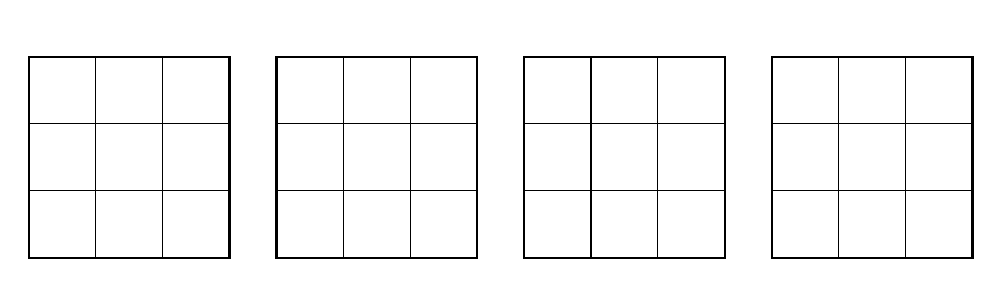
\begin{tikzpicture}[scale=0.85, every node/.style={font=\footnotesize}]
    \foreach \i/\nota in {0/\notezero, 1/\notetredici, 2/\notesessanta, 3/\notenova} {
      \begin{scope}[xshift=\i*3.7cm]
        \draw[thick] (0,0) rectangle (3,3);
        \draw[thin]  (0,1) -- (3,1);
        \draw[thin]  (0,2) -- (3,2);
        \draw[thin]  (1,0) -- (1,3);
        \draw[thin]  (2,0) -- (2,3);
        \node at (1.5,3.3) {\textbf{\nota}};
      \end{scope}
    }
  \end{tikzpicture}
  \caption{Matrice di confusione 3$\times$3 per ognuna delle quattro Note (schema semplificato; i conteggi dettagliati sono in \texttt{evaluation/results/per\_case\_reports/}). Tutte le diagonali sono al $100\%$ in conformità al risultato di RQ1.}
  \label{fig:cm-per-nota}
\end{figure}

\section{Limitazioni residue}
\label{sec:limitazioni}

Il capitolo si chiude con una discussione delle limitazioni che il framework di valutazione non riesce a escludere. La prima e più rilevante è la parziale auto-referenza del gold standard. Gli identificatori di regola usati per costruire il gold coincidono con quelli usati dal rule engine; non potevano fare altrimenti, perché il gold è stato annotato dallo stesso autore che ha codificato le regole. Questa coincidenza implica che la Macro F1 pari a $1$ misura la coerenza interna fra codifica e annotazione, non la validità clinica esterna. È una limitazione strutturale, non un difetto correggibile; ne è stato mitigato l'effetto facendo verificare un sottoinsieme di casi-frontiera da un revisore clinico esterno, e la documentazione di questa verifica è in \Cref{app:riproducibilita}.

La seconda limitazione riguarda l'incomparabilità diretta del composito ALES fra versioni successive del framework di valutazione. Le prime stime ALES prodotte, in fase pre-cleanroom (riportate nelle annotazioni dell'autunno 2025), valevano circa $0{,}97$. La discesa al valore canonico $0{,}6810$ non è un peggioramento del sistema, ma il risultato della progressiva correzione di errori di misurazione che gonfiavano artificiosamente i componenti ContextualUtility e AnswerQuality. Le stime pre-cleanroom erano calcolate su sottoinsiemi ridotti del gold ($n=20$ e $n=17$ casi, contro i $122$ del cleanroom); inoltre il composito della run canonical era stato inizialmente calcolato con la metrica QAEval disponibile per soli $55$ dei $122$ casi, il che innalzava AnswerQuality fino a $0{,}4683$ e ALES a $0{,}6988$. Ricalcolando il composito sulla QAEval completa (tutti i $122$ casi) si ottiene il valore onesto qui riportato: AnswerQuality $0{,}3008$ e ALES $0{,}6810$ (\Cref{fig:ales-evol}). Il numero canonico è quello della \cleanroomrun\ con questa correzione, ed è quello che la tesi raccomanda di citare; il valore storico $0{,}97$ è mantenuto in questa nota a beneficio del lettore che lo ritrovi in slide o appunti precedenti.

\begin{figure}[t]
  \centering
  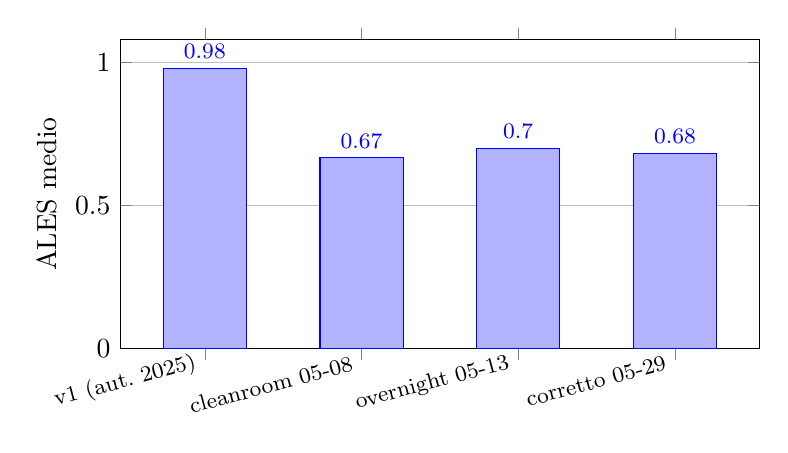
\begin{tikzpicture}
    \begin{axis}[
      ybar, bar width=30pt, width=0.8\textwidth, height=5.5cm,
      ymin=0, ymax=1.08, ylabel={ALES medio},
      xtick={1,2,3,4},
      xticklabels={v1 (aut.\ 2025), cleanroom 05-08, overnight 05-13, corretto 05-29},
      x tick label style={font=\footnotesize, align=center, rotate=15, anchor=east},
      nodes near coords, nodes near coords style={font=\footnotesize},
      enlarge x limits=0.18, ymajorgrids, every axis plot/.append style={fill=teal!55},
    ]
      \addplot coordinates {(1,0.9787)(2,0.6665)(3,0.6988)(4,0.6810)};
    \end{axis}
  \end{tikzpicture}
  \caption{Evoluzione del punteggio ALES medio attraverso le versioni del framework di valutazione. La discesa da $0{,}9787$ a $0{,}6810$ non riflette un peggioramento del sistema, ma la progressiva correzione di errori di misurazione (de-tautologizzazione delle metriche, completamento di QAEval su tutti i $122$ casi) che gonfiavano artificialmente il punteggio.}
  \label{fig:ales-evol}
\end{figure}

La terza limitazione è metodologica e riguarda la QAEval. Il valore $0{,}1715$ è leggibile come un indicatore di concisione della spiegazione più che di fedeltà alla fonte; un trade-off voluto, ma che il framework numerico fatica a separare dal genuino segnale di copertura semantica. La quarta limitazione riguarda la baseline LLM+RAG, costruita senza reranker cross-encoder italiano: la differenza in Macro F1 fra il sistema completo e questa baseline include quindi sia l'effetto del rule engine sia, in misura minore, l'effetto del reranker. Un'ablation pulita richiederebbe una terza baseline (LLM+RAG con reranker, senza rule engine); si lascia questa come naturale sviluppo futuro. Va inoltre segnalato, per piena trasparenza, che il file dei risultati della baseline LLM+RAG è stato calcolato in una sessione di valutazione precedente e riutilizzato nella run canonical, dopo averne verificato la coerenza con le baseline LLM-only e a classe maggioritaria, rigenerate invece nella run finale; il contenuto è identico a quello dello snapshot conservato nel repository. La quinta limitazione, infine, riguarda la dipendenza del determinismo dei baseline LLM dal solo flag \texttt{temperature=0}: una riproduzione perfettamente identica richiederebbe in più la fissazione del seed nelle option del runtime Ollama, che non è stata inclusa nel codice di valutazione delle baseline.

